%%%%%%%%%%%%%%%%%%%%%%%%%%%%%%%%%%%%%%%%%
% Journal Article
% LaTeX Template
% Version 2.0 (February 7, 2023)
%
% This template originates from:
% https://www.LaTeXTemplates.com
%
% Author:
% Vel (vel@latextemplates.com)
%
% License:
% CC BY-NC-SA 4.0 (https://creativecommons.org/licenses/by-nc-sa/4.0/)
%
% NOTE: The bibliography needs to be compiled using the biber engine.
%
%%%%%%%%%%%%%%%%%%%%%%%%%%%%%%%%%%%%%%%%%

%----------------------------------------------------------------------------------------
%	PACKAGES AND OTHER DOCUMENT CONFIGURATIONS
%----------------------------------------------------------------------------------------

\documentclass[
	a4paper, % Paper size, use either a4paper or letterpaper
	10pt, % Default font size, can also use 11pt or 12pt, although this is not recommended
	unnumberedsections, % Comment to enable section numbering
	twoside, % Two side traditional mode where headers and footers change between odd and even pages, comment this option to make them fixed
]{LTJournalArticle}

\addbibresource{bib.bib} % BibLaTeX bibliography file

\runninghead{} % A shortened article title to appear in the running head, leave this command empty for no running head

\footertext{} % Text to appear in the footer, leave this command empty for no footer text

\setcounter{page}{1} % The page number of the first page, set this to a higher number if the article is to be part of an issue or larger work

%----------------------------------------------------------------------------------------
%	TITLE SECTION
%----------------------------------------------------------------------------------------

\title{Embedding GitHub Issues for Optimal Retrieval} % Article title, use manual lines breaks (\\) to beautify the layout

% Authors are listed in a comma-separated list with superscript numbers indicating affiliations
% \thanks{} is used for any text that should be placed in a footnote on the first page, such as the corresponding author's email, journal acceptance dates, a copyright/license notice, keywords, etc
\author{%
	Ilan Aliouchouche, Ekaterina Timofeeva, Nikshep Grampurohit
    % \textsuperscript{1,2}, Robert Smith\textsuperscript{3} and Jane Smith\textsuperscript{1}\thanks{Corresponding author: \href{mailto:jane@smith.com}{jane@smith.com}\\ \textbf{Received:} October 20, 2023, \textbf{Published:} December 14, 2023}
}

% Affiliations are output in the \date{} command
% \date{\footnotesize\textsuperscript{\textbf{1}}School of Chemistry, The University of Michigan\\ \textsuperscript{\textbf{2}}Physics Department, The University of Wisconsin\\ \textsuperscript{\textbf{3}}Biological Sciences Department, The University of Minnesota}

% Full-width abstract
% \renewcommand{\maketitlehookd}{%
% 	\begin{abstract}
% 		\noindent DO WE WRITE SMTH HERE? alskdalskfmalsdkfslkdmflskdmflskdmflskdmflskdmflskd sldkfsmldkfms dlfksmdlkfmsldkf sdlkfmsdfbh
% 	\end{abstract}
% }

%----------------------------------------------------------------------------------------

\begin{document}

\maketitle % Output the title section

%----------------------------------------------------------------------------------------
%	ARTICLE CONTENTS
%----------------------------------------------------------------------------------------

\section{Introduction}

Duplicate issues in Git repositories waste time and fragment discussions. To solve this, we propose different models to assist in searching for issues using embedding-based search. By computing vector embeddings of issues, we enable efficient similarity searches.

A key use case is automated duplicate detection: when a new issue is pushed, its embedding is compared against existing ones. If a match is found, the user is prompted to review the existing thread instead of creating a duplicate. This improves issue tracking, streamlining collaboration and reducing repository noise.

 


%------------------------------------------------

\section{Dataset}
Many duplicate issues are observed on GitHub. Typically, open source organizations maintainers tend to mark these duplicate issues as closed with a comment such as 'closing as a duplicate of \#id'. Consequently, these duplicate issues inherently serve as a source for the STS task. It is also worth noting that most issues contain long texts because of the inclusion of extensive code within the issues. 

To compile the data set~\autocite{li-li-2024-aoe}, the authors extracted duplicated issues from 55 popular open source projects on GitHub using the GitHub API. Duplicate issues were used as positive samples, while the remaining issues were considered negative samples. Table~\ref{tab:github_statistics} presents statistics of the GitHub Issues Similarity Dataset~\footnote{\url{https://huggingface.co/datasets/WhereIsAI/github-issue-similarity}}.

\begin{table}[h]
    \centering
    \caption{Statistics of the proposed GitHub Issues Similarity Dataset. \#Positive denotes the count of positive pairs, and \#Negative represents the number of negative pairs.}
    \label{tab:github_statistics}
    \begin{tabular}{lccc}
        \toprule
        Split & Train & Validation & Test \\
        \midrule
        \#Positive & 9457 & 774 & 807 \\
        \#Negative & 9108 & 773 & 741 \\
        \midrule
        Total & 18565 & 1547 & 1548 \\
        \bottomrule
    \end{tabular}
\end{table}

%------------------------------------------------

\section{Exploratory Data Analysis}
The primary goal of this EDA was to gain initial insight into the structure and characteristics of the GitHub issue similarity dataset. This understanding is essential to inform subsequent modeling decisions. Table~\ref{tab:token_length} shows the average length of tokens across train, validation and test sets.

\begin{table}[h]
    \centering
    \caption{Average token length across training, validation, and test sets.}
    \label{tab:token_length}
    \begin{tabular}{ccc}
        \toprule
         Train & Validation & Test \\
        \midrule
         540.58& 516.90& 452.22\\
    \end{tabular}
\end{table}

The github issues have HTML tags, which makes the data very variable in size and may not have any relation to the actual content of the issue. Therefore, we decided to remove HTML tags from the dataset. The number of tokens per sample distribution before and after the removal of HTML tags is presented in Table~\ref{fig:enter-label}.

\begin{figure}[!h]
    \centering
    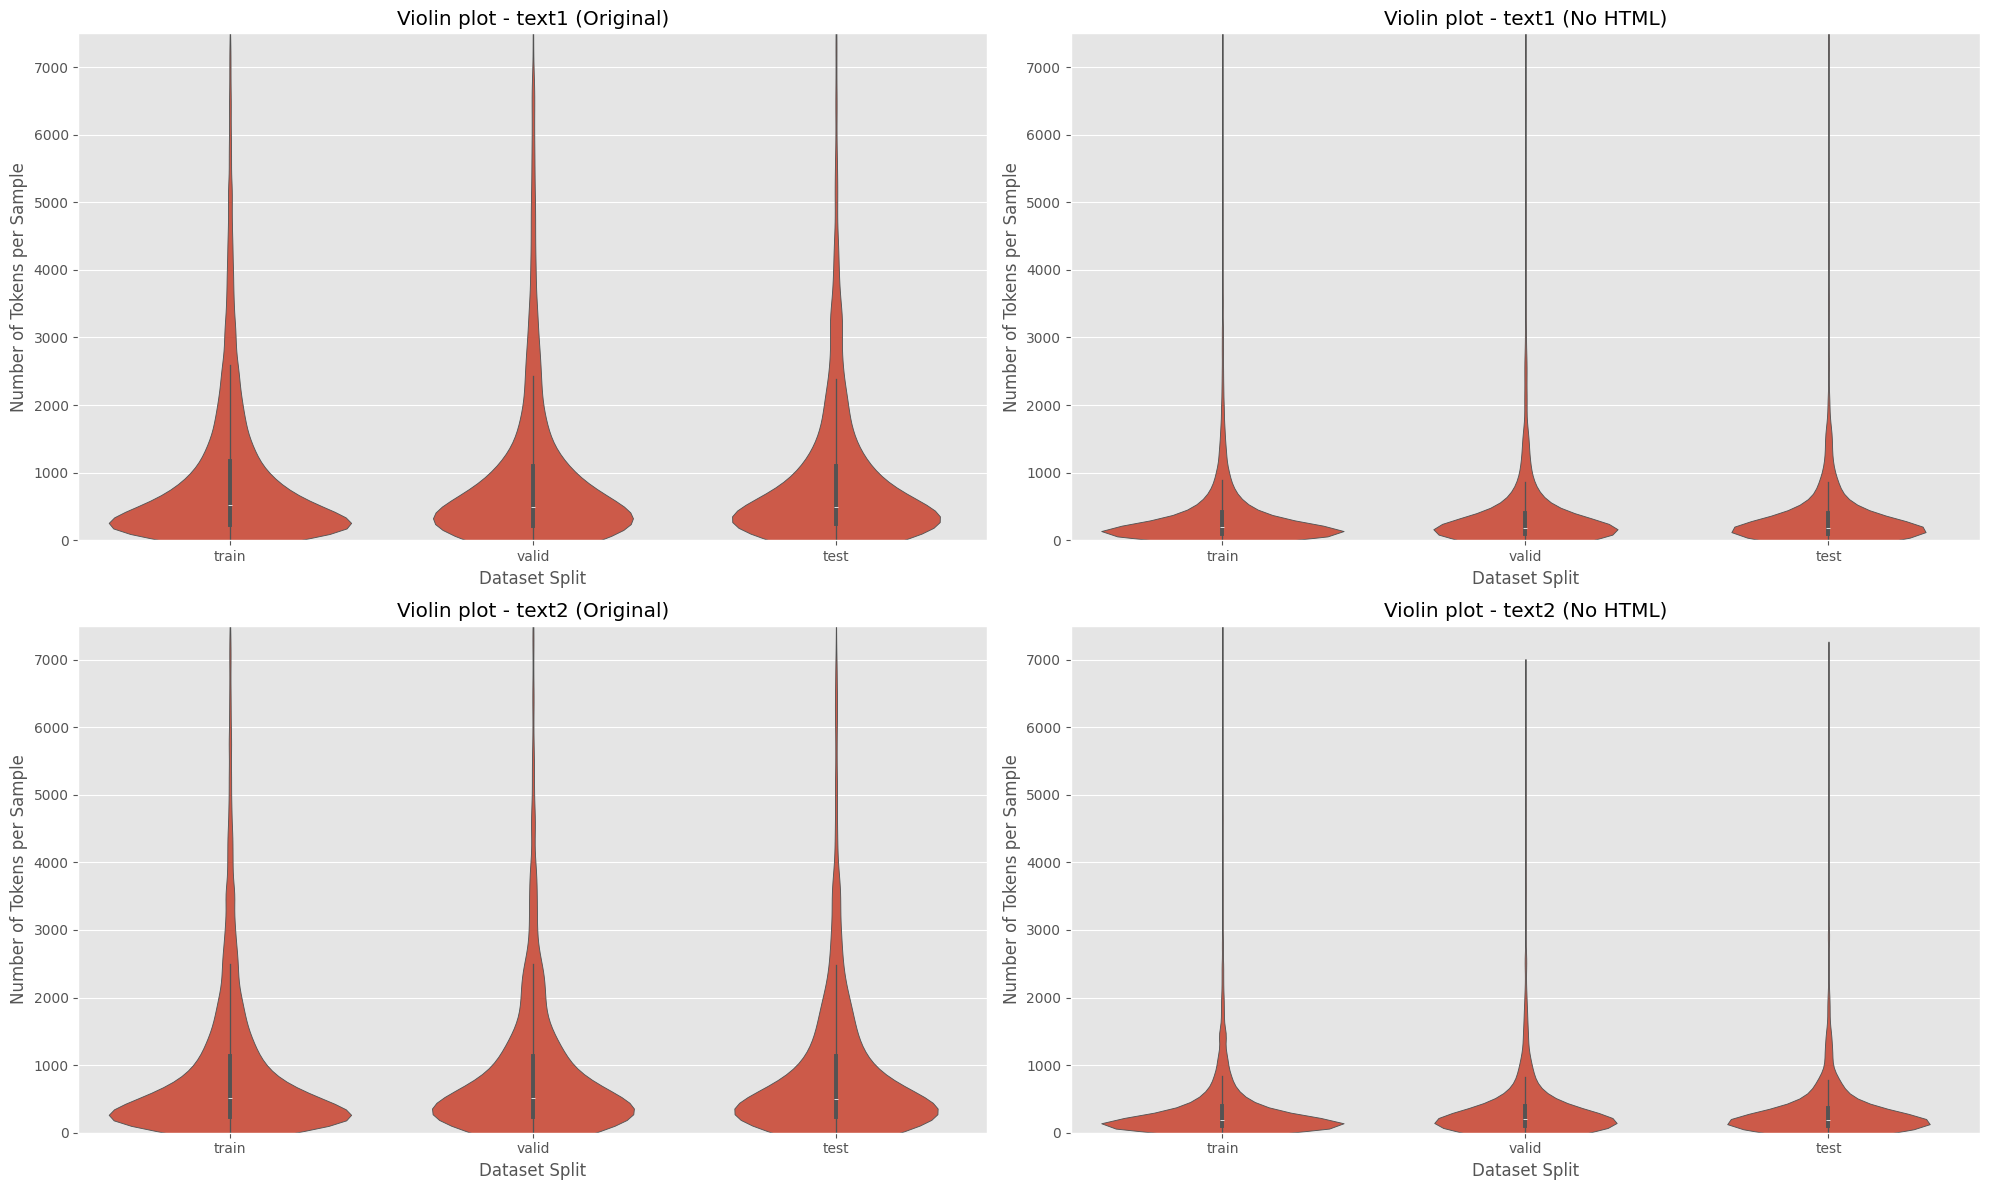
\includegraphics[width=0.75\linewidth]{violin.png}
    \caption{Number of tokens per sample distribution before and after removing HTML tags.}
    \label{fig:enter-label}
\end{figure}
%------------------------------------------------
\section{Models}

\subsection{Jasper and Stella model}
The Jasper and Stella models~\autocite{stella} are advanced text embedding models developed to enhance dense retrieval tasks, such as those found in FAQ systems and Retrieval-Augmented Generation (RAG). These models aim to balance performance with computational efficiency, making them suitable for deployment in various applications. Jasper is a student model with 2 billion parameters, built upon the Stella~\footnote{\url{https://huggingface.co/NovaSearch/stella_en_400M_v5}} embedding model. It incorporates model distillation to achieve high performance while maintaining a manageable model size.

\subsection{GTE}
The GTE models~\autocite{gte} are trained by Alibaba DAMO Academy. They are mainly based on the BERT framework and currently offer three different sizes of models, including GTE-large, GTE-base, and GTE-small~\footnote{\url{https://huggingface.co/prdev/mini-gte}}. The GTE models are trained on a large-scale corpus of relevance text pairs, covering a wide range of domains and scenarios. This enables the GTE models to be applied to various downstream tasks of text embeddings, including information retrieval, semantic textual similarity, text reranking, etc.

\subsection{Multilingual E5 text embedding model}
The Multilingual E5 model~\autocite{e5} is a state-of-the-art text embedding model developed by Microsoft, designed to handle multiple languages and various tasks such as passage retrieval and semantic similarity. Based on the XLM-RoBERTa-large architecture, the multilingual-e5-small~\footnote{\url{https://huggingface.co/intfloat/multilingual-e5-small}} model comprises 12 layers, generating 384-dimensional embeddings. The model was trained using contrastive pre-training on 1 billion multilingual text pairs, followed by fine-tuning on a combination of labeled datasets. Supports 100 languages, making it a versatile tool for tasks involving multiple languages.

%------------------------------------------------
\section{Loss functions}

\subsection{Contrastive Loss}
The contrastive loss function~\autocite{contrastive} is commonly used to train models that learn to distinguish between similar and dissimilar data points. The contrastive loss function is defined as:

\[
L = (1 - Y) \cdot D^2 + Y \cdot \max(0, m - D)^2
\]

where:
\begin{itemize}
    \item \( Y \) is 0 if the pair is \textbf{similar}, 1 if \textbf{dissimilar}
    \item \( D \) is the Euclidean distance between embeddings
    \item \( m \) is a \textbf{margin} that ensures dissimilar pairs are separated by at least \( m \)
\end{itemize}
\subsection{Online contrastive Loss}
Online Contrastive Loss is an extension of the traditional contrastive loss function, designed to improve efficiency in training deep learning models by dynamically selecting informative pairs from a larger dataset. Instead of using random pairs, it actively selects the most useful samples, reducing computational redundancy. It selects hard positive (positives that are far apart) and hard negative pairs (negatives that are close) and computes the loss only for these pairs.

\subsection{Multiple Negative Ranking Loss}
Multiple Negatives Ranking (MNR) Loss~\autocite{mnrl} is a contrastive learning technique commonly used in self-supervised learning and retrieval-based tasks. Instead of comparing only one negative sample at a time (like contrastive loss), MNR loss compares multiple negative examples in a batch, making training more efficient and improving generalization.

\subsection{Cached Multiple Negatives Symmetric Ranking Loss}
The Cached Multiple Negatives Symmetric Ranking Loss (CMNSRL)~\autocite{cmnsrl} is an advanced loss function designed to enhance the training of sentence embeddings by leveraging both in-batch negatives and a caching mechanism. This approach is particularly useful in scenarios where large batch sizes are computationally expensive or infeasible.

%------------------------------------------------

\section{Results}

TODO: Write here



%----------------------------------------------------------------------------------------
%	 REFERENCES
%----------------------------------------------------------------------------------------

\printbibliography % Output the bibliography

%----------------------------------------------------------------------------------------


\end{document}
